\documentclass{article}
\usepackage[utf8]{inputenc}
\usepackage{graphicx,psfrag}
\usepackage{mathrsfs}
\usepackage{amsmath,amsfonts,amssymb}
\usepackage{multirow}
\usepackage{comment}
\usepackage{ulem}
\usepackage{hyperref}
\usepackage{enumitem}
\usepackage{multirow}
\usepackage{morefloats}
\usepackage{appendix}
\usepackage{hyperref}
\usepackage{hyperref}
\usepackage{geometry}
\usepackage{color}


\newcommand{\todo}[1]{\textcolor{red}{$\blacksquare$ TODO: #1}} 

\geometry{a4paper, tmargin=2cm, bmargin=2cm, lmargin=1cm, rmargin=1cm, headheight=2em, headsep=2em, footskip=1cm}

\title{test}
\author{fizik.vlk }
\date{November 2019}

\begin{document}

\maketitle

\section{Solution of the initial boundary value problem with the wave equation}
\subsection{Write down the general analytical solution of the IVP. Note it is composed of two \textit{elementary waves}}
Given: \\
\begin{equation}\label{eq:waveq:2}
\partial_{tt} \phi - c^2 \partial_{xx} \phi = 0  \ ,
\end{equation}

Solution: \\
\begin{equation}
	(\partial_t - c\partial_x)(\partial_t + c\partial_x)\phi(x,t) = 0
\end{equation}
Chose new variable: \\
\begin{equation}
	\begin{aligned}
	\lambda = x + ct \\
	\eta = x - ct
	\end{aligned}
\end{equation}
That relate to old ones as,
\begin{equation}
	\begin{aligned}
	\lambda + \eta = 2x \\
	\lambda - \eta = 2ct
	\end{aligned}
\end{equation}
%
\begin{equation}
	\begin{aligned}
	x = \frac{\lambda + \eta}{2} \\
	t = \frac{\lambda - \eta}{2 t}
	\end{aligned}
\end{equation}
Computing derivatives,
\begin{equation}
	\begin{aligned}
	\partial_x &= \frac{\partial\lambda}{\partial x}\frac{\partial}{\partial\lambda} + \frac{\partial\eta}{\partial x}\frac{\partial}{\partial \eta} = \frac{\partial}{\partial\lambda} + \frac{\partial}{\partial\eta} \\
	\partial_t &= \frac{\partial \lambda}{\partial t}\frac{\partial}{\partial \lambda} + \frac{\partial \eta}{\partial t}\frac{\partial}{\partial \eta} = c\frac{\partial}{\partial \lambda} - c\frac{\partial}{\partial \eta} 
	\end{aligned}
\end{equation}
Putting them back into the equation \ref{eq:waveq:2},
\begin{equation}
(c\partial_{\lambda} - c\partial_{\eta} - c\partial_{\lambda} -c\partial_{\eta})(c\partial_{\lambda} -c\partial_{\eta}+c\partial_{\lambda}+c\partial_{\eta})\phi(\lambda,\eta) = 0
\end{equation}
simplifying, 
\begin{equation}
	\partial_{\eta}\partial_{\lambda} \phi(\lambda,\eta) = 0
\end{equation}
This is a well known equation, that has a general solution of form:
\begin{equation}
	\phi(\lambda,\eta) = F(\lambda) + G(\eta)
\end{equation}
or
\begin{equation}
	\label{eq:waveq:gensol}
	\phi(x,t) = F(x-ct) + G(x+ct)
\end{equation}
that can be interpreted as two \textit{elementary waves}.
%
%
%
\subsection{Rewrite the wave equation from the second order form above to a	first-order in time and second-order in space system}
The goal of this exercise is to recognize that the differential equation that is second order in time and space, e.g. Eq. \ref{eq:waveq:2} can be reduced to a system of coupled equation, first order in time, using the substitution:
\begin{equation}
	\begin{aligned}
	\partial_t\phi &= \Pi \\
	\partial_t\Pi &= c^2\partial_{xx}\phi
	\end{aligned}
\end{equation}
%
It is also possible to express the solution as a function of the initial data, to show that the solution of the wave equation is the advection equation, that describes a propagation of the initial data. \\
%
Given also the initial data as $\phi(x,0)=\theta(x)$, which putting into the solution above \ref{eq:waveq:gensol}, obtaining: $\theta(x) = F(x) + G(x)$, derivative of which is:

\begin{equation}
	\partial_x\theta(x) = cF'(x) - cG'(x) = \psi(x)
\end{equation}
where we defined $\psi(x)$ at the last step. \\
Integrating, we obtain:
\begin{equation}
	cF(x) - cG(x) = \frac{1}{c}\int_{x_0}^{x}\psi(x')dx' + K
\end{equation}
%
where $K$ is a constant of integration. \\
Substitute this into the $F(x) = \theta(x) - G(x)$:
\begin{equation}
	\theta(x) - G(x) -G(x) = \frac{1}{c}\int_{x_0}^{x}\psi(x')dx' + K
\end{equation}
%
\begin{equation}
	G(x) = \frac{1}{2} - \frac{1}{2c}\int_{x_0}^{x}\psi(x')dx' + K
\end{equation}
Using $F(x) = \theta(x) - G(x)$ again, we obtain,
\begin{equation}
	F(x) = \frac{1}{2}\theta(x) + \frac{1}{2c}\int_{x_0}^{x}\psi(x')dx' + K
\end{equation}
Substituting $x \rightarrow x+ct$ in $F$ and $x\rightarrow x-ct$ in $G$, obtain
\begin{equation}
	\begin{aligned}
	\phi(x,t) &= F(x+ct) + G(x-ct) = \\
	&= \frac{1}{2}\theta(x+ct) + \frac{1}{2c}\int_{x_0}^{x+ct}\psi(x')dx'-K + \frac{1}{2}\theta(x-ct) + \frac{1}{2c}\int_{x_0}^{x-ct}\psi(x')dx' = \\
	&= \frac{1}{2}\Big(\theta(x+ct)+\theta(x-ct)\Big)+\frac{1}{2c}\int_{x_0}^{x+ct}\psi(x')dx'+\frac{1}{2c}\int_{x-ct}^{x_0}\psi(x')dx' = \\
	&= \frac{1}{2}\Big(\theta(x+ct)+\theta(x-ct)\Big)+\frac{1}{2c}\int_{x-ct}^{x+ct}\psi(x')dx'
	\end{aligned}
\end{equation}
This is the generic solution, if the initial profile is given. 

\todo{What a student should discuss here? What are the 2 choses for $\Pi(t=0,x)$}
 
\subsection{Write the wave equation as a fully first order system by defining the new variables}
Given: \\
\begin{equation}
	\begin{aligned}
	\partial_{tt}\phi - c^2\partial_{xx}\phi &= 0 \\
	\partial_t\Pi &= c^2 \partial_x
	\end{aligned}
\end{equation}
Introduce $\partial_t\phi=\chi$, thus $\partial_t\partial_x\phi=\partial_t\chi$,assuming that $\partial_t$ and $\partial_x$ commute, and $\partial_x = \partial_t\chi$. \\
Together, $\phi$, $\Pi$, $\chi$ form a special state-vector. 
\begin{equation}
	\label{eq:waveq:vectorstate}
	\begin{aligned}
	\partial_t\phi &= \Pi \\
	\partial_t\Pi &= c^2\partial_x\chi \\
	\partial_t\chi &= \partial_x\Pi
	\end{aligned}
\end{equation}
which can be expressed in a matrix form
\begin{equation}
	\begin{pmatrix}
	\partial_t\phi \\
	\partial_t\Pi \\
	\partial_t\chi
	\end{pmatrix} 
	+ 
	\begin{pmatrix}
	0 & 0 & 0 \\
	0 & 0 & -c^2 \\
	0 & -1 & 0 
	\end{pmatrix}
	\begin{pmatrix}
	\partial_x\phi \\
	\partial_x\Pi \\
	\partial_x\chi
	\end{pmatrix}
	=
	\begin{pmatrix}
	\Pi \\
	0 \\
	0
	\end{pmatrix}
\end{equation}
defining the state vector
\begin{equation}
	u = 
	\begin{pmatrix}
	\phi \\ 
	\Pi \\
	\chi
	\end{pmatrix}
\end{equation}
, matrix as $A$ and rhs of the equation as $S$, we obtain a system that is equivalent to wave equation
\begin{equation}
	\partial_t u + A\partial_x u = S
\end{equation}
%
First note, that the matrix $A$ is degenerate, containing row of $0$s. Taking the principle part of wave equation, sub-block of $A$:
\begin{equation}
	\tilde{A} =
	\begin{pmatrix}
	0 & -c^2 \\
	-1 & 0
	\end{pmatrix}
\end{equation}
we can obtain eigenvalues and convectors, 
\begin{equation}
	|\tilde{A} - \bar{E}\lambda| = 0
\end{equation}
%
\begin{equation}
	\begin{pmatrix}
	0 & -c^2 \\
	-1 & 0
	\end{pmatrix}
	-
	\begin{pmatrix}
	\lambda & 0 \\
	0, & \lambda
	\end{pmatrix}
	= 0
\end{equation}

\begin{equation}
	\begin{pmatrix}
	-\lambda & -c^2 \\
	-1 & -\lambda
	\end{pmatrix}
	= 0
\end{equation}
\begin{equation}
	\lambda^2 - c^2 = 0 \rightarrow \lambda = \pm c
\end{equation}
Eigenvectors are found as 
\begin{equation}
	A\upsilon = \lambda\upsilon
\end{equation}
let 
\begin{equation}
	\upsilon = 
	\begin{pmatrix}
	x \\
	y
	\end{pmatrix}
\end{equation}
then
\begin{equation}
	\begin{pmatrix}
	0 & -c^2 \\
	-1 & 0
	\end{pmatrix}
	\begin{pmatrix}
	x \\ 
	y
	\end{pmatrix}
	= \lambda
	\begin{pmatrix}
	x \\
	y
	\end{pmatrix}
\end{equation}
or equivalently,
\begin{equation}
	\begin{aligned}
	-c^2y &= \lambda x \\
	-x &= \lambda y
	\end{aligned}
\end{equation}
As there is a freedom of choice, we can set $x=c$ and $y=1$ for $\lambda=-c$, and $x=-c$, $y=1$ for $\lambda=c$.
this the matrix of eigenvectors is 
\begin{equation}
	R = (\upsilon_1, \upsilon_2) = 
	\begin{pmatrix}
	c & -c \\
	1 & 1
	\end{pmatrix}
\end{equation}
which can be verified by performing 
\begin{equation}
	AR = R\Lambda
\end{equation}
The $\Lambda$ is a diagonal matrix. Thus, overall, using $w := Ru$, the wave-equation \ref{eq:waveq:2} was reduced to a diagonal (decoupled) system. Equivalently, this is a set of advection, transport equations. 

\todo{Is this all that a student should present for analytical part?}

\section{Finite differentiating approximation}
\label{sec:findiffapp}
Principle: derivatives in the partial differential equations are approximated by linear combinations of function values at the grid points. \\
In 1D we define set of equally spaced grid points $x_i = i\Delta x$ with $i = 0 ... n-1$ and $\Delta x = 1 / (n-1)$ that discretizes the domain $\Omega = (0, 1)$. To compute the derivatives in this framework, consider the definition of a first order derivative
\begin{equation}
	\frac{\partial u}{\partial x}(x) = \lim\limits_{\Delta x \rightarrow 0}\frac{u(\bar{x}+\Delta x) - u(\bar{x})}{\Delta x} = \lim\limits_{\Delta x \rightarrow 0} \frac{\bar{u}(x) - u(\bar{x} - \Delta x)}{\Delta x} = \lim\limits_{\Delta x \rightarrow 0}\frac{u(\bar{x} + \Delta x) - u(\bar{x} - \Delta x)}{2\Delta x}
\end{equation}
Geometrically, the 
\begin{equation}
	\Big(\frac{\partial u}{\partial x}\Big)_i \approx \frac{u_{i+1} - u_i}{\Delta x}
\end{equation}
is a forward difference,
\begin{equation}
\Big(\frac{\partial u}{\partial x}\Big)_i \approx \frac{u_i - u_{i-1}}{\Delta x}
\end{equation}
-- backward difference and
\begin{equation}
\Big(\frac{\partial u}{\partial x}\Big)_i \approx \frac{u_{i+1} - u_{i-1}}{2\Delta x}
\end{equation}
is a central difference.
To asses the level of approximation, consider a Taylor series:
\begin{equation}
	\begin{aligned}
	u(x) &= \sum\limits_{n=0}^{\infty} = \frac{(x-x_i)^n}{n!}\Big(\frac{\partial^n u}{\partial x^n}\Big)_i, \hspace{5mm} u\in(|0,1|) \\
	u_{i+1} &= u_i \textcolor{red}{+} \Delta x\Big(\frac{\partial u}{\partial x}\Big)_i + \frac{(\Delta x)^2}{2}\Big(\frac{\partial^2 u}{\partial x^2}\Big)_i + \frac{(\Delta x)^3}{6}\Big(\frac{\partial^3 u}{\partial x^3}\Big)_i + ... \\
	u_{i-1} &= u_i \textcolor{red}{-} \Delta x\Big(\frac{\partial u}{\partial x}\Big)_i + \frac{(\Delta x)^2}{2}\Big(\frac{\partial^2 u}{\partial x^2}\Big)_i + \frac{(\Delta x)^3}{6}\Big(\frac{\partial^3 u}{\partial x^3}\Big)_i + ... 
	\end{aligned}
\end{equation}
Analysis of a truncation errors 
\begin{equation}
	\begin{aligned}
	T_1 &\Rightarrow \Big(\frac{\partial u}{\partial x}\Big)_i = \frac{u_{i+1} - u_i}{\Delta x} - \textcolor{red}{\frac{\Delta x}{2}\Big(\frac{\partial^2 u}{\partial x^2}\Big)_i - \frac{(\Delta x)^2}{6}\Big(\frac{\partial^3 u}{\partial x^3}\Big)_i + ...} \\
	T_2 &\Rightarrow \Big(\frac{\partial u}{\partial x}\Big)_i = \frac{u_i - u_{i-1}}{\Delta x} + \textcolor{red}{\frac{\Delta x}{2}\Big(\frac{\partial^2 u}{\partial x^2}\Big)_i - \frac{(\Delta x)^2}{6}\Big(\frac{\partial^3 u}{\partial x^3}\Big)_i + ...} \\
	T_1 - T_2 &\Rightarrow \Big(\frac{\partial u}{\partial x}\Big)_i + \frac{u_{i+1} - u_{i-1}}{2\Delta x} - \textcolor{red}{ \frac{(\Delta x)^2}{6}\Big(\frac{\partial^3 u}{\partial x^3}\Big)_i + ... } 
	\end{aligned}
\end{equation}
with the first term on the right hand side being the central difference and the second, red, being the truncation error $O(\Delta x)^2$ \\
Leading truncation error can be expressed as 
\begin{equation}
	\epsilon_r = \alpha_m(\Delta x)^m + \alpha_{m+1}(\Delta x)^{m+1} + ... \approx \alpha_m(\Delta x)^m
\end{equation}
%
Consider second derivative, the finite differencing formulation can be similarly obtained, 
\begin{equation}
	T_1 + T_2 \Rightarrow \Big(\frac{\partial^2 u}{\partial x^2}\Big)_i + \frac{u_{i+1} - 2u_i +  u_{i-1}}{(\Delta x)^2} - \textcolor{red}{ \frac{(\Delta x)^2}{24}\Big(\frac{\partial^4 u}{\partial x^4}\Big) + ... } 
\end{equation}
with the first term on the right hand side being the central difference and the second, red, being the truncation error $O(\Delta x)^2$ \\
Alternatively, the second derivative can be derived as,
\begin{equation}
\begin{aligned}
	\Big(\frac{\partial^2 u}{\partial x^2}\Big)_i = \Big[\frac{\partial}{\partial x}\Big(\frac{\partial u}{\partial x}\Big)\Big]_i & = \lim\limits_{\Delta x \rightarrow 0}\Big[\Big(\frac{\partial u}{\partial x}\Big)_{i+1/2} - \Big(\frac{\partial u}{\partial x}\Big)_{i-1/2}\Big] \Big/\Delta x \\
	& \approx \Big[\frac{u_{i+1} - u_i}{\Delta x} - \frac{u_i - u_{i-1}}{\Delta x}\Big] \Big/ \Delta x = \frac{u_{i+1} - 2u_i + u_{i-1}}{(\Delta x)^2}
\end{aligned}
\end{equation}

Examples. Consider an analytical faction and its derivatives:
\begin{equation}
	\label{func:ex1}
	\begin{aligned}
	f(x) = \Big(x - \frac{1}{2}\Big)^2 + x \hspace{5mm}
	f'(x) = 2x \hspace{5mm}
	f''(x) = 2 
	\end{aligned}
\end{equation}
\begin{equation}
\label{func:ex2}
\begin{aligned}
f(x) = \Big(x - \frac{1}{2}\Big)^3 + \Big(x-\frac{1}{2}\Big)^2 + x \hspace{5mm}
f'(x) = 3x^2 -x + \frac{3}{4} \hspace{5mm}
f''(x) = 6x - 1
\end{aligned}
\end{equation}
\begin{equation}
\label{func:ex3}
\begin{aligned}
	f(x) = \sqrt{x} \hspace{5mm}
	f'(x) = \frac{1}{2\sqrt{x}} \hspace{5mm}
	f''(x) = - \frac{1}{4 x^{3/2}}
\end{aligned}
\end{equation}
\begin{equation}
\label{func:ex4}
\begin{aligned}
f(x) = \sin(12\pi x) \hspace{5mm}
f'(x) = 12\pi\cos(12\pi x) \hspace{5mm}
f''(x) = 1 = -144\pi\sin(12\pi x)
\end{aligned}
\end{equation}
\begin{equation}
\label{func:ex5}
\begin{aligned}
f(x) &= \sin^4(12\pi x) \\ 
f'(x) &= 48 \pi \cos(12 \pi x) \sin^3(12 \pi x)  \\
f''(x) &=  -576 \pi^2 \sin^2(12 \pi x) (-3 \cos^2(12 \pi x) + \sin^2(12 \pi x))
\end{aligned}
\end{equation}
\begin{equation}
\label{func:ex6}
\begin{aligned}
f(x) &= \exp(-a x^2) \\ 
f'(x) &= -2 a \exp(-a x^2) x  \\
f''(x) &=  2 a \exp(-a x^2) (-1 + 2 a x^2)
\end{aligned}
\end{equation}

\subsection{Numerical implementation}
See script \texttt{ex1.py} for the code. \\
In this code see the function \texttt{findif(f, n, x1, x2, ord, acc, method)}, that performs the finite differencing of a function $f(x)$, using $n$ equally spaced points between $x1$ and $x2$, using the stencil of order $ord$ and accuracy $acc$ with method $method$. \\
Possible orders: $[1,2]$ for the first and second order derivative \\
Possible accuracies: $[2,4]$ for the second and 4th order accuracy stencils \\
Possible methods: $ghost$, $onesided$. The first one will extend the $x$ to 1 (2) points in left and right for second (forth) accuracies and computes the central finite differencing for points between $0$ to $n$, using added points as ghosts. Second method uses one-sided stencils for 1 (2) border points, where central stencil cannot be used. \\
To write stencils the coefficients from \url{https://en.wikipedia.org/wiki/Finite_difference_coefficient} were used. \\
%  
To study the convergence consider norm:
\begin{equation}
	\begin{aligned}
	||x||_p = \sqrt[p]{\sum x_i ^p} 
	\end{aligned}
\end{equation}
From the previous analysis, 
\begin{equation}
	f' _E(x) - f' _h(x) = Ch^2 + O(h^3)
\end{equation}
where $f' _E(x)$ is an analytical derivative, exact solution, and $f' _h(x)$ is a numerical derivative with spacing $h$.  Thus,
\begin{equation}
	\frac{||f' _E(x) - f' _h(x)||_2}{||f' _E - f' _{h/2}(x)||_2} = \frac{Ch^{\theta}}{C(h/2)^{\theta}} = \frac{h^{\theta}}{h^{\theta}}\times 2^{\theta} = 2^{\theta}
\end{equation}
if this equation holds, the convergence is achieved. \\
If the analytic solution $f' _E(x)$ is not available, the self-convergence test can be performed, using 3 (or more) resolutions in a following manner:
\begin{equation}
\frac{||f' _h(x) - f' _{h/2}(x)||_2}{||f' _{h/2} - f' _{h/4}(x)||_2} = 2^{\theta}
\end{equation}
Using special function for the test \texttt{convergence(f, df, ddf)}, that takes the actual function $f(x)$, its first analitical derivative $df(x)$ and second $d(df(x))$ perform the convergence test. \\
%
\begin{figure}[t]
	\centering 
	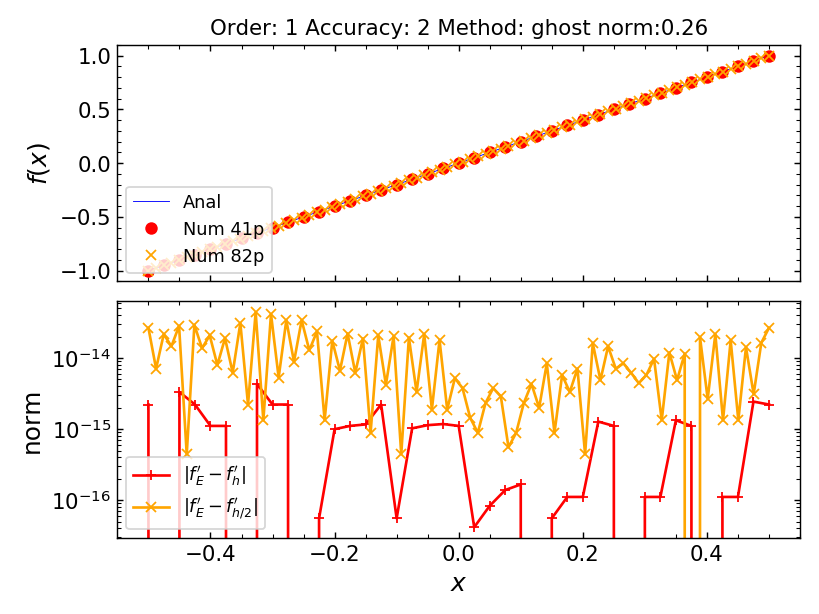
\includegraphics[width=0.32\textwidth]{./fig/f1_1_2_ghost.png}
	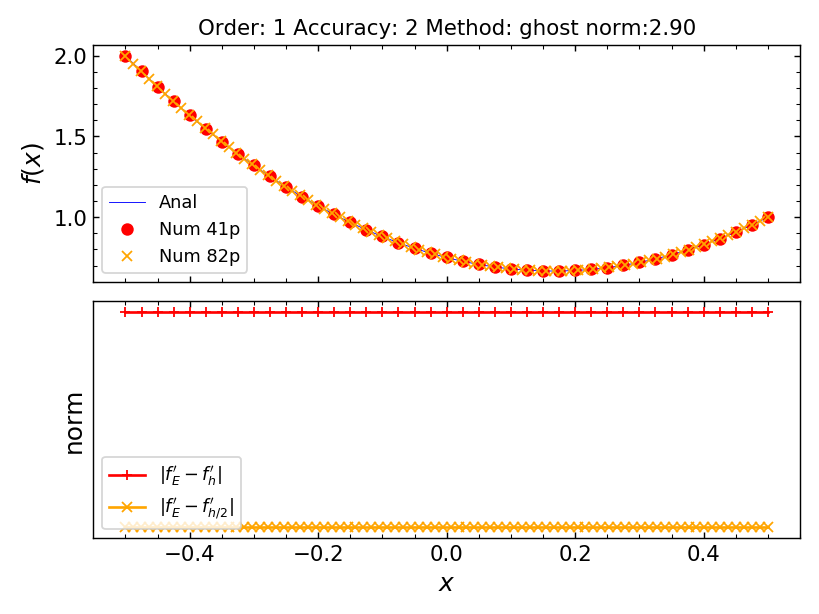
\includegraphics[width=0.32\textwidth]{./fig/f2_1_2_ghost.png}
	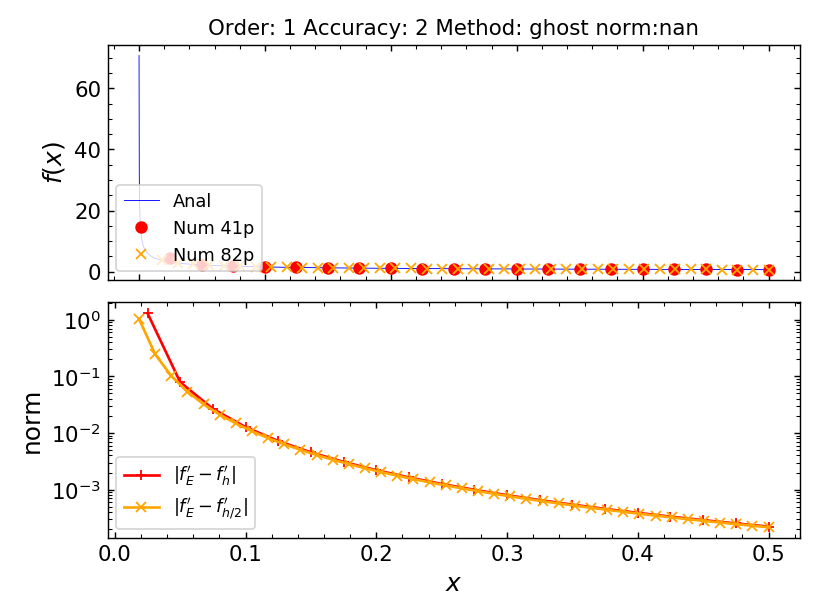
\includegraphics[width=0.32\textwidth]{./fig/f3_1_2_ghost.png}
	%
	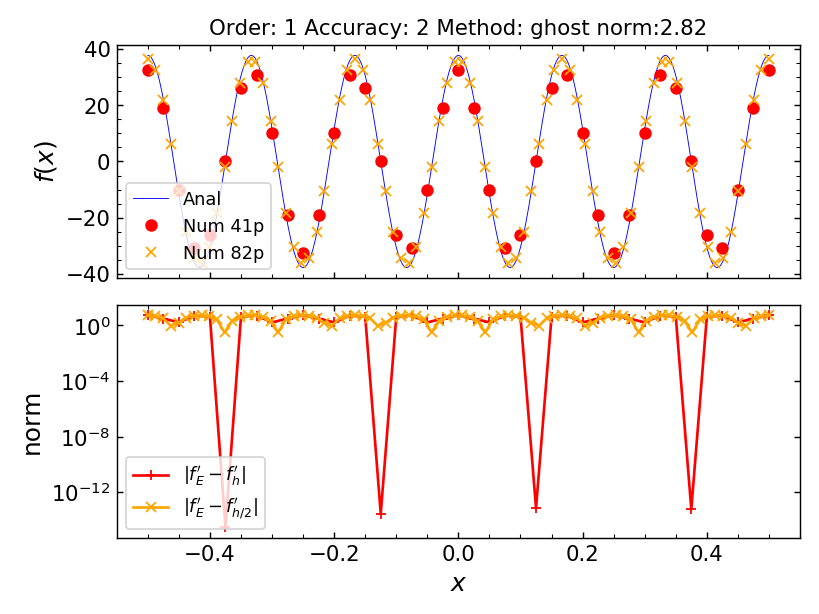
\includegraphics[width=0.32\textwidth]{./fig/f4_1_2_ghost.png}
	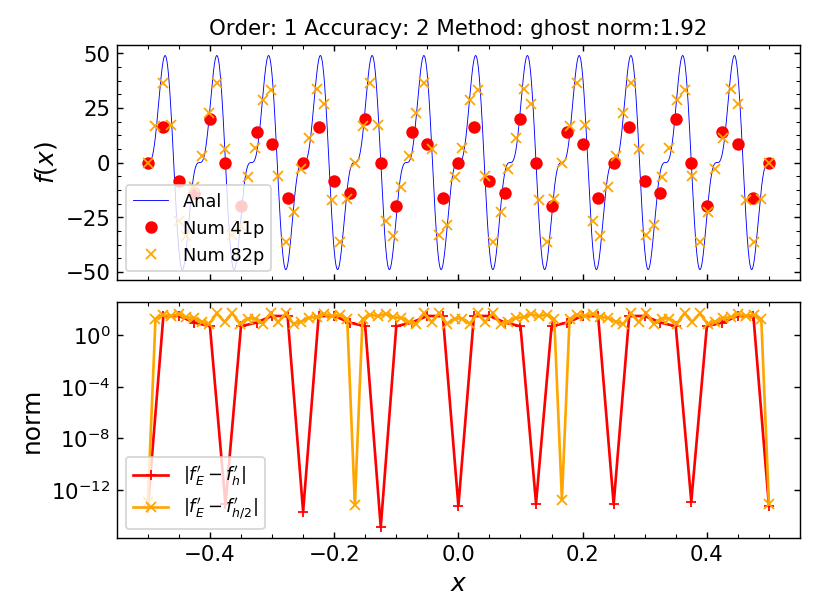
\includegraphics[width=0.32\textwidth]{./fig/f5_1_2_ghost.png}
	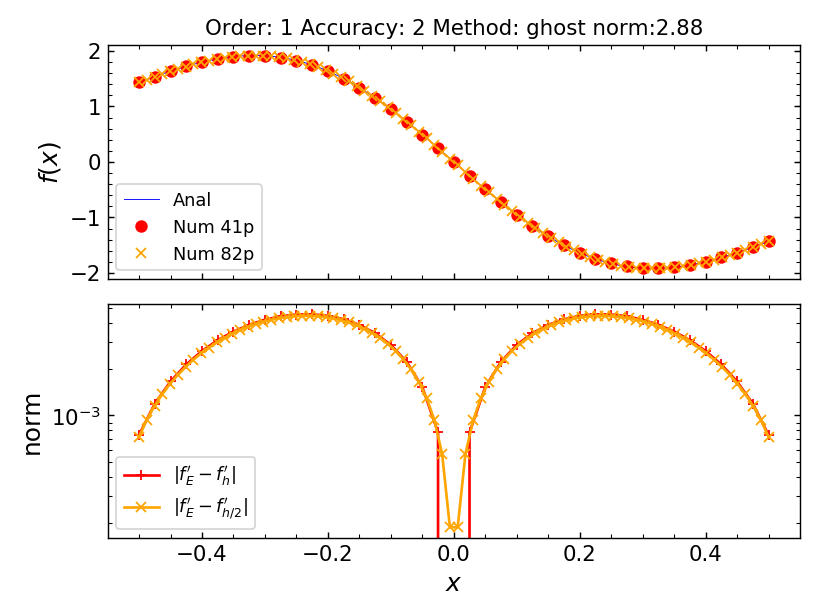
\includegraphics[width=0.32\textwidth]{./fig/f6_1_2_ghost.png}
	\caption{
		First derivatives, using ghosts and convergence tests
	}
	\label{fig:conv1}
\end{figure}
%
Fig. \ref{fig:conv1} shows the first derivative computed using 2order accuracy stencil (with 2 ghosts) and the convergence for all 6 functions  \ref{func:ex1}, \ref{func:ex2}, \ref{func:ex3}, \ref{func:ex4}, \ref{func:ex5}, \ref{func:ex6}. For second order derivatives, 4th order stencil and self-convergence see plots in \texttt{/WaveProject/fig/}.

\subsection{Runge-Kutta time-integration}

Consider the harmonic oscillator. Its Hamiltonian is
\begin{equation}
	H(q.p) = \frac{1}{2}\Big(\frac{p^2}{m} - q^2m \Big), \hspace{5mm} q = \omega x
	\label{eq:harm_oscill_h}
\end{equation} 
One can also introduce the constant $k$ such that, $\omega = \sqrt{k/m}$. The period of oscillation is $T=2\pi/\omega$. \\
Fo simplicity consider $\omega = 1$, thus, $T=2\pi$. \\
This transforms the equation \ref{eq:harm_oscill_h} to:
%
\begin{equation}
	2H = p^2 + x^2 \hspace{5mm} \text{(a const.)}
\end{equation}

Hence, a trajectory in the "phase space" plot, i.e. trajectory in the $x-p$ plane, should be a circle of radius $\sqrt{2E}$.\\
The Newton's equation of motion are is \textcolor{red}{I strongly believe that this equation has to be given in the excessive. I did not get, that I have to solve this one} 
\begin{equation}
	\frac{\partial^2 x}{\partial t^2} = -x
\end{equation}
which can be written as a two first order differential equations 
\begin{equation}
	\begin{aligned}
	\frac{\partial x}{\partial t} &= p, \\
	\frac{\partial p}{\partial t} &= -x
	\end{aligned}
\end{equation}
These equations can be solved analytically as well as numerically. \\
First consider an analytical solution, (where we restored $\omega$) which is 
\begin{equation}
	x(t) = C_1 \exp(-t\sqrt{-\omega}) + C_2 \exp(t\sqrt{-\omega})
\end{equation}
setting initial conditions allows to obtain constants $C_1$, $C_2$,
\begin{equation}
	\begin{aligned}
	C_1 + C_2 &= x_0, \\
	-C_1 \sqrt{-\omega} + C_2\sqrt{-\omega} &= \upsilon_0
	\end{aligned}
\end{equation}
where $\upsilon_0$ and $x_0$ are initial position and coordinate. Solving this system, gives
\begin{equation}
	\begin{aligned}
	C_1 = -\frac{\upsilon_0}{2\sqrt{-\omega}} + \frac{x_0}{2}, \\
	C_2= \frac{\upsilon_0}{2\sqrt{-\omega}} + \frac{x_0}{2}
	\end{aligned}
\end{equation}
and thus, the overall solution is 
\begin{equation}
	x(t) = \Big(-\frac{\upsilon_0}{2\sqrt{-\omega}}+\frac{x_0}{2}\Big)\exp(-t\sqrt{-\omega}) + \Big(\frac{\upsilon_0}{2\sqrt{-\omega}} + \frac{x_0}{2}\Big)\exp(t\sqrt{-\omega})
	\label{eq:harm_oscil_sol}
\end{equation}
This generic solution can be simplified for two cases. \\
First. Initial position is $x_0 = 0$ and initial velocity $\upsilon_0\neq 0$. This reduces the Eq. \ref{eq:harm_oscil_sol} to 
\begin{equation}
	x(t) = \cos(t)
\end{equation}
Second. initial position is zero and initial velocity is nonzero:
\begin{equation}
	x(t) = -\frac{i}{2}e^{it} + \frac{i}{2}e^{-it}
\end{equation}
which is equivalent to $\sin(x)$.
Proceeding to the numerical solution, see the implementation in script \texttt{ex2.py} \\
The 4-th order Runge-Kutta time-integration is implemented following following \url{https://www.youtube.com/watch?v=mqoqAovXxWA&t=4s}. There is not need in finite-differencing techniques in the exercise. The result of this implementation is shown in Fig. \ref{fig:harm_oscil_num_sol}

\begin{figure}[t]
	\label{fig:harm_oscil_num_sol}
	\centering 
	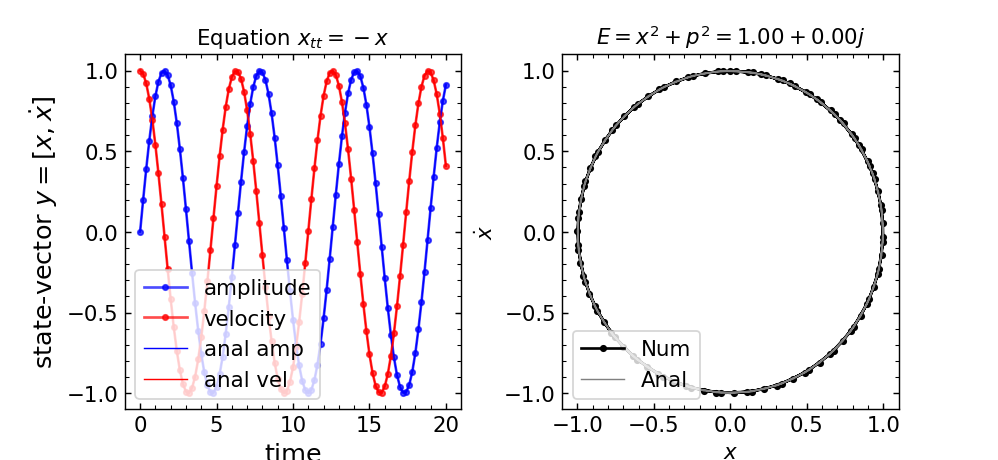
\includegraphics[width=0.82\textwidth]{./fig2/harmonic_oscillator.png}
	\caption{Numerical and analytical solutions to  the harmonic oscillator for the coordinate and its velocity on the left and for energy on the right.}
\end{figure}

Parameters used are $x_0=0$ $p_0=1$, $t_0=0$, $t_{max}=20$, $h=0.2$ and constants were set to $m=1$, $\omega=1$. \\
Convergence and energy conservation are showen in \ref{fig:harm_oscil_conv}.

\begin{figure}[t]
	\label{fig:harm_oscil_conv}
	\centering 
	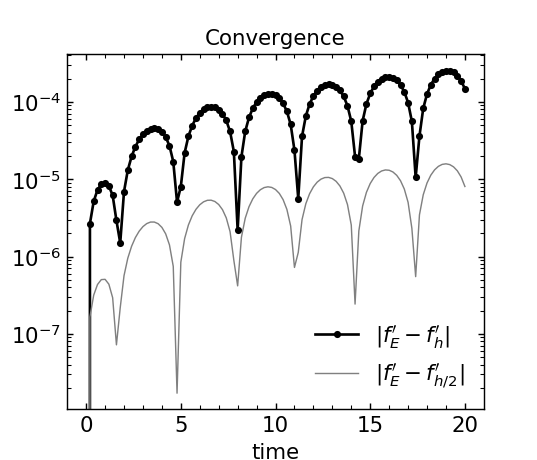
\includegraphics[width=0.32\textwidth]{./fig2/convergence_harm_osc.png}
	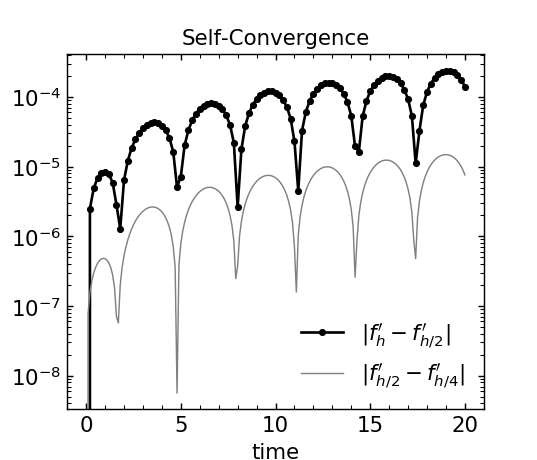
\includegraphics[width=0.32\textwidth]{./fig2/self-convergence_harm_osc.png}
	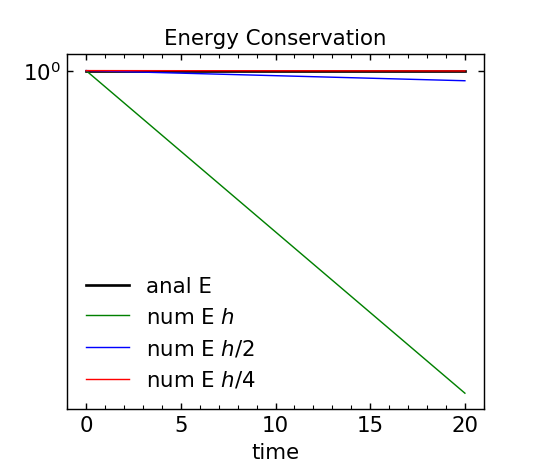
\includegraphics[width=0.32\textwidth]{./fig2/energy_conservation.png}
	\caption{Convergence, self-convergence and energy conservation of the numerical implementation of the harmonic oscillator}
\end{figure}

Overall, as expected, the convergence of the problem is $>16$ (for $4th$ order Runge-Kutta time-integration due to symmetries. However, self-convergence is lower and is $12$. This might be due to low resolution $h$. The energy conservation is present to a high order, but the system is loosing energy with time, and the energy loss is the highest for low resolution $h$.

\section{Wave Equation}
Consider the reduced to a 1st order in time wave equation:
\begin{equation}
\begin{aligned}
\partial_t\phi &= \Pi \\
\partial_t\Pi &= c^2\partial_{xx}\phi
\end{aligned}
\end{equation}
For the time derivative the Runge-Kutta scheme can be implemented in accordance with the previous exercise. For the spatial derivative $\partial_{xx}\phi$ the finite diferencing can be used in accordance with the section \ref{sec:findiffapp}, which will transform the system to a semi-analytic system:
\begin{equation}
\begin{aligned}
\partial_t\phi &= \Pi \\
\partial_t\Pi &= c^2 \frac{\phi_{i+1} - 2\phi_i +  \phi_{i-1}}{(\Delta x)^2}
\end{aligned}
\end{equation}
where $\phi_{i}$, $\phi_{i+1}$, $\phi_{i-1}$ are the values of the function at a grid point $i$, $i+1$ and $i-1$, $\Delta x$ is the grid spacing. This is the \textit{method of lines}. \\
%
As was discussed in the section \ref{sec:findiffapp}, for the central stencil of the finite diferencing method, points around the $i$ are required. At the boundaries of the grid, for example from $i=0$ to $i=n$, method requires points at $i=-1$ and $i=n+1$, that are not part of physical domain. The solution here is to use so-called \textit{ghost points}, extending the actual domain of the solution to include the required points. Thus the physical domain would lay in range $i\in[ng, N-ng]$, where $ng$ is the number of ghost points ($1$ for the first order accuracy schemes and $2$ for the second), and $N$ is the total number of points. \\
In the case of the second order PDE, the boundary condition has to be specified. Here the \textit{periodic boundary conditions} are implemented as a following. \\
In its core, the periodic boundary conditions imply that at the boundaries of the domain that condition in imposed such that $\phi[0]=\phi[n]$. However, implementing such a condition would lead to numerical complications, such as the difficulty with filling the ghost points. Another approach lays in a considering the grid as a \textit{staggered grid} (see fig. \ref{fig:grid}). This leads to the boundary conditions beiing realized as shown in the left panel of the fig. \ref{fig:grids}.
\begin{figure}[t]
	\label{fig:grids}
	\centering 
	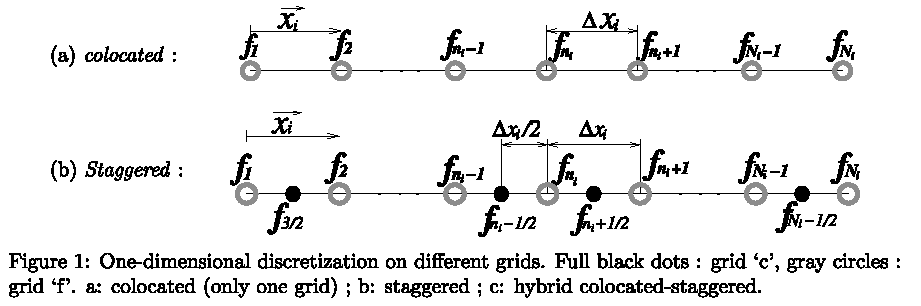
\includegraphics[width=0.42\textwidth]{./fig3/grids.pdf}
	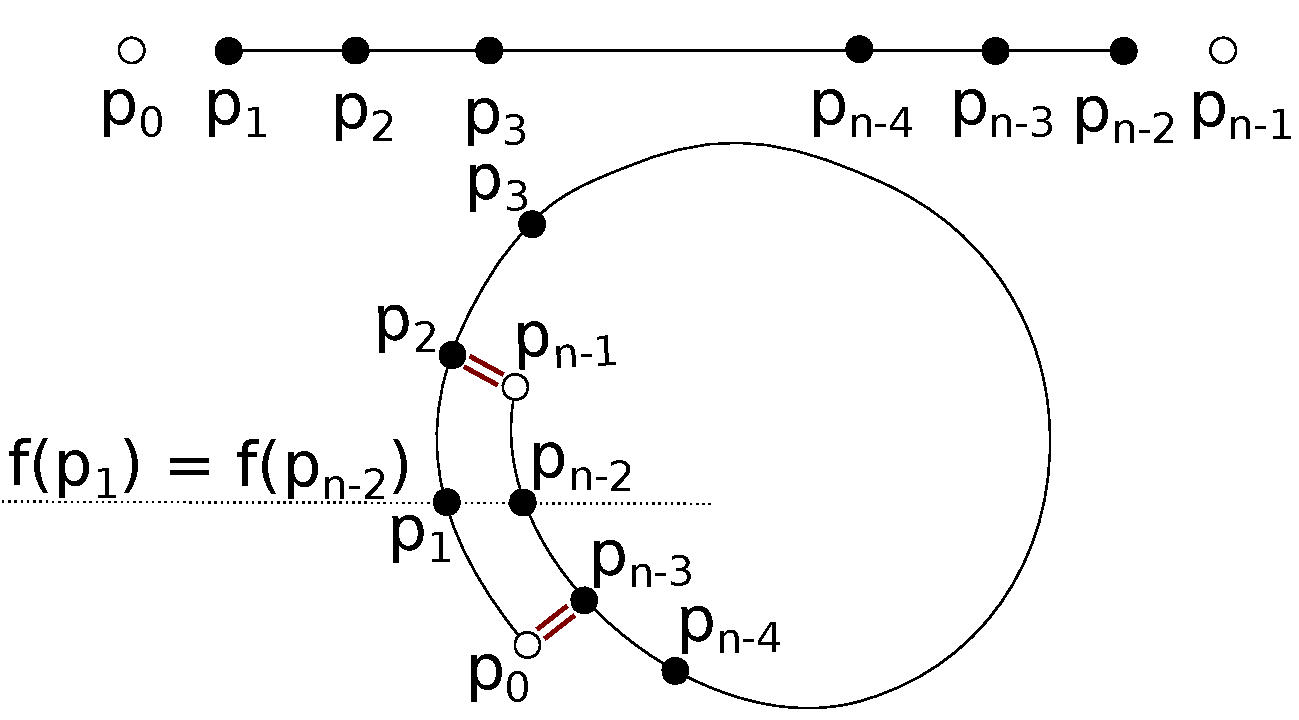
\includegraphics[width=0.42\textwidth]{./fig3/cartoon.pdf}
	\caption{Different grid types, staggered grid periodic boundary conditions for the staggered grid on the right. Here, filled dots are of physical domain. Unfilled -- ghost points.}
\end{figure}
there, the condition that $f(p_{1}) = f(p_{n-2})$, the function is the same at the last physical points of the grid on the left and on the right is assured by setting ghosts $p_0$ and $p_{n-1}$ to their respective values on the other side, namely: 
\begin{equation}
\begin{aligned}
f(p_{n-1}) = f(p_2) \\
f(p_{0}) = f(p_{n-3})
\end{aligned}
\end{equation}
Now, having the equations, methods to solve (Runge-Kutta and finite differencing) and methods to implement boundary conditions, the numerical implementation can be realized. The last thing is to fix the initial profile, the $\phi_0$ and $\Pi_0 = \partial/\partial_t\phi_0$. Consider first the simple periodic function:
\begin{equation}
\begin{aligned}
\phi &= \cos(2 \pi (x-t))
\end{aligned}
\end{equation}, 
The initial profile is
\begin{equation}
\begin{aligned}
\phi_0 &= \cos(2 \pi x) \\
\Pi_0 &= 2\pi\sin(2 \pi x)
\end{aligned}
\end{equation},
With initial profile, the numerical implementation yields the following results (see \texttt{ex3.py} for the code): 
\begin{figure}[t]
	\label{fig:grids}
	\centering 
	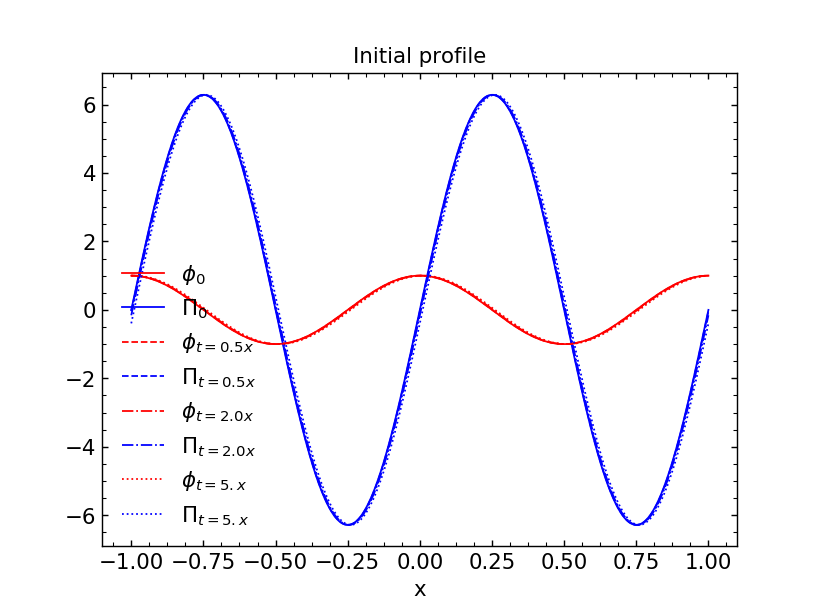
\includegraphics[width=0.42\textwidth]{./fig3/inital_profile.png}
	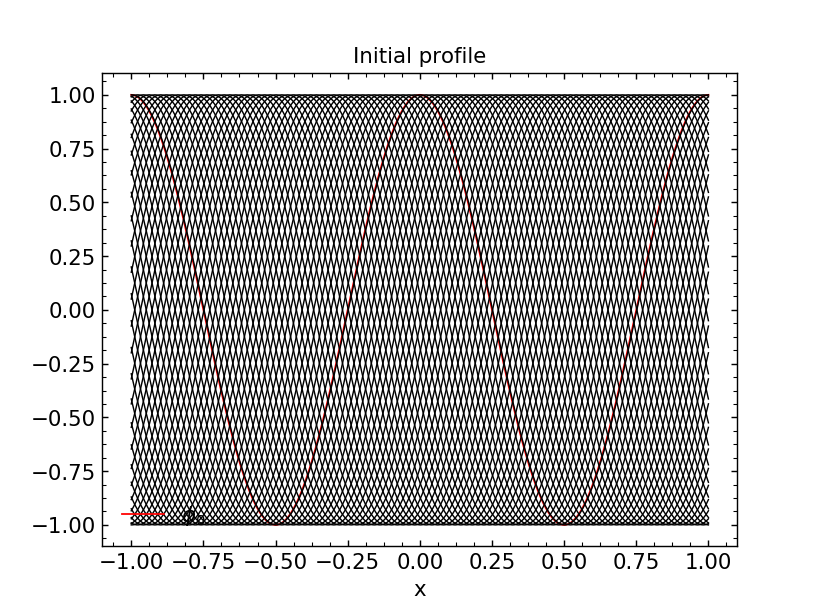
\includegraphics[width=0.42\textwidth]{./fig3/wave_propagation_1d.png}
	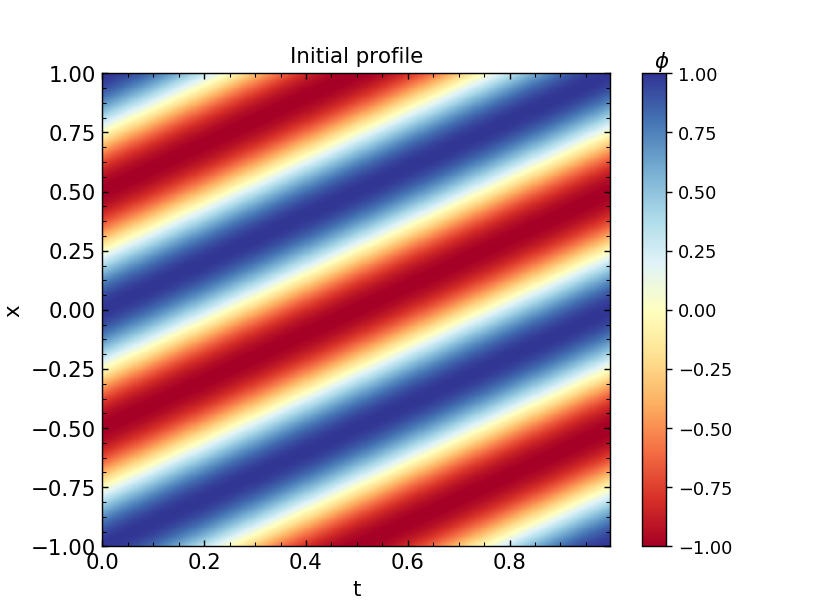
\includegraphics[width=0.42\textwidth]{./fig3/wave_propagation_colomesh.png}
	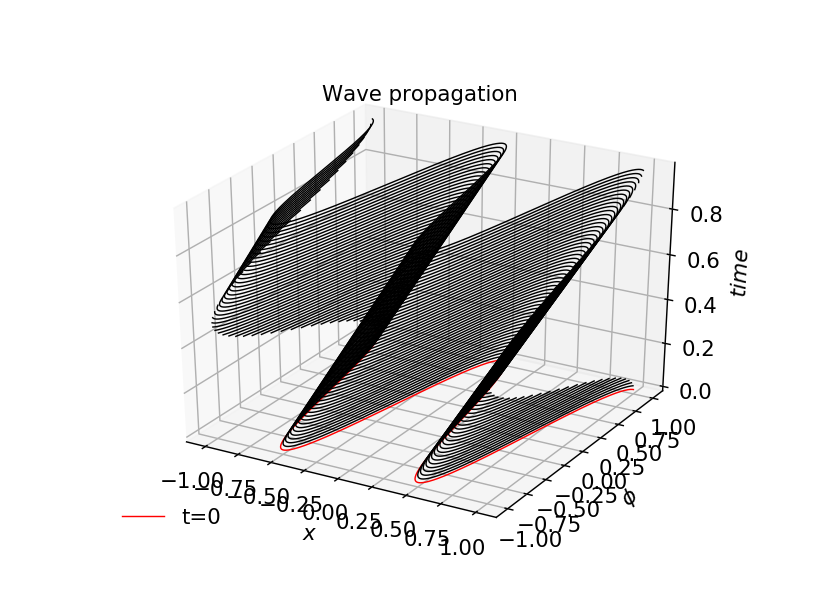
\includegraphics[width=0.42\textwidth]{./fig3/wave_propagation_3d.png}
	\caption{Right top panel -- initial profile with different $dt$ steps. It shows that with current $N$ or $dx$ settings, the effect of higher timestep is small. Top left panel -- initial profile for $\phi_0$ and its time evolution untill $t=1.$ with timestep $dt=0.5dx$ to assure stability. Bottom left panel -- time evolution of the $\phi$ colorcoded as a function of $x$ and $t$. See peaks of the waves moving along $x$ with time. Bottom left -- same, but a 3D plot.}
\end{figure}

\section{Convergence of the numerical implementation of the Wave Equation}
%
\begin{figure}[t]
	\label{fig:wave_profiles}
	\centering 
	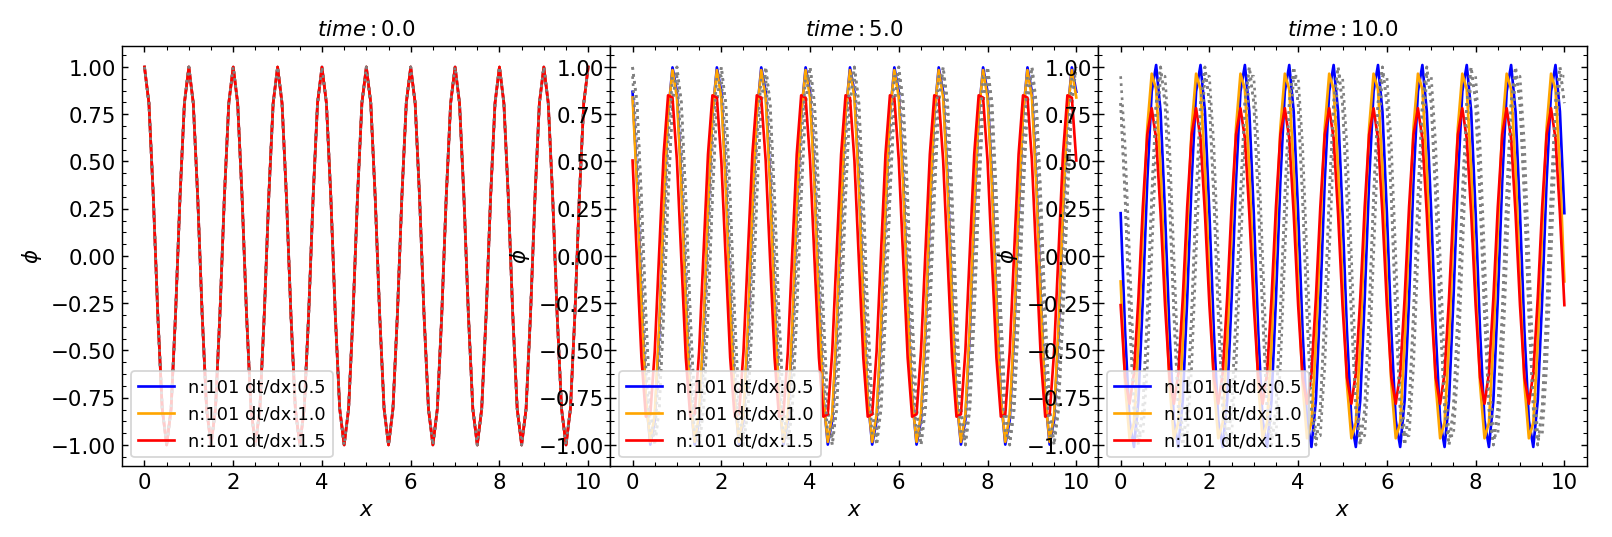
\includegraphics[width=0.92\textwidth]{./fig4/profiles.png}
	\caption{Comparison of the solution at three timepsteps and three values of $dt/dx$. Used coursed grid of $101$ points}
\end{figure}
%
Fig. \ref{fig:wave_profiles} shows that with time the solution changes due to numerical dissipation. The effect intensifies for higher $dt/dx$. At $dt/dx$ the evolution becomes unstable.
%
See \url{https://hplgit.github.io/fdm-book/doc/pub/wave/pdf/wave-4print.pdf} for a very good description of the process. 
Assessing convergence of the numerical scheme, the familiar formula is utilized:
\begin{equation}
\frac{||f' _E(x) - f' _h(x)||_2}{||f' _E - f' _{h/2}(x)||_2} = \frac{Ch^{\theta}}{C(h/2)^{\theta}} = \frac{h^{\theta}}{h^{\theta}}\times 2^{\theta} = 2^{\theta}
\end{equation}
In the numerical implementation (see script \texttt{ex4.py}) the grid density is set as $n$, which in turn sets the spacing $dx$. The evolution timestep is set via the $dt = \xi dx$. Equivalently, in terms of spacing is $\Delta t = (\alpha / |c|) h = \xi h$. \\
Taking for the convergence study $n_1 = 101$ and $n_2 = 201$, twice as much, and the $\xi=1.$ results not only in having twice as dens spatial grid, but also in having twice as many time steps for the evolution, to preserve the $\xi=1.$ This is important fact not to overlook. \\
To compute convergence, the follwoing quantities are to be estimated $f'_{E}(x)$, $f'_{h}(x)$, $f'_{h/2}(x)$ for the equation 
\begin{equation}
norm = \log_2\Bigg( \frac{||f' _{E}(x) - f' _h(x)||_2}{||f' _E(x) - f' _{h/2}(x)||_2}\Bigg)
\end{equation}
or in terms of $n$: $f'_{E,n}(x)$, $f'_{n}(x)$, $f'_{2n}(x)$. However, to compute the denominator, $f'_{E,n}(x) - f'_{2n}(x)$, either analytic solution has to be recomputed with the $2n$ grid or take half of the array of numerical solution $f'_{2n}(x)$. Taking the first approach the, numerically the \textit{norm} is estimated as 
\begin{equation}
norm = \log_2\Bigg( \frac{\sqrt{\sum( f' _{E;n}(x) - f' _{n}(x))^2}}{\sqrt{\sum( f' _{E;2n}(x) - f' _{2n}(x))^2}}\Bigg)
\label{eq:conv_num}
\end{equation}
Computing this norm for every timespte (of the solution with $n$ grid and every second timestep for the solution with $2n$ points), result is shown in the fig
\begin{figure}[t]
	\label{fig:conv_wave_eq}
	\centering 
	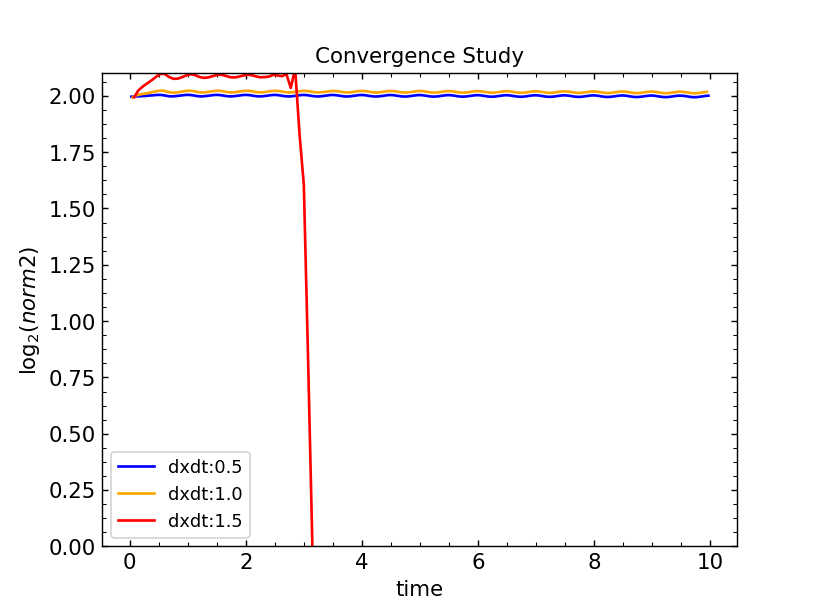
\includegraphics[width=0.42\textwidth]{./fig4/convergence_dxdt.png}
	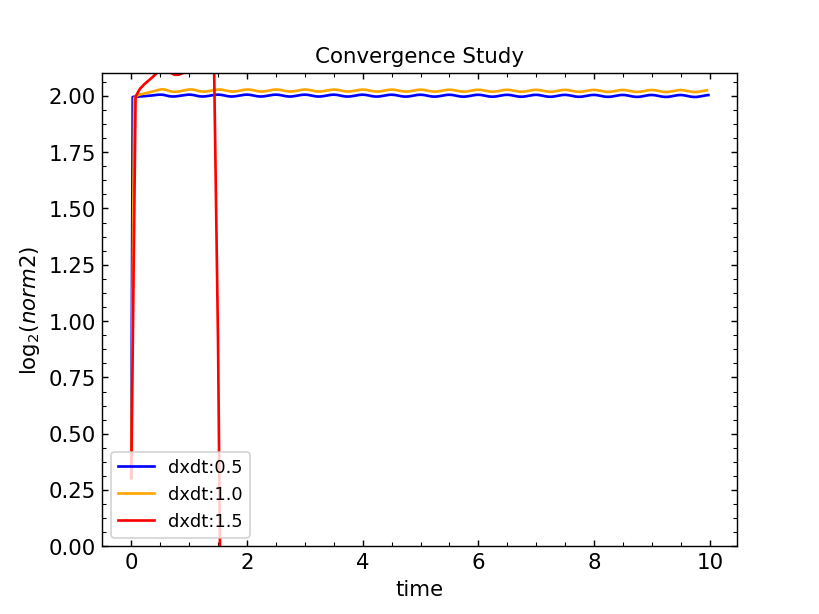
\includegraphics[width=0.42\textwidth]{./fig4/self_convergence_dxdt.png}
	\caption{Convergence (left) and self-convergence(right) study. Plotted $\log_2(norm2)$ from eq. \ref{eq:conv_num} as a function of time. Three $dx/dt$ are shown. }
\end{figure}
Similarly, the self-convergence is computed (Fig.\ref{fig:conv_wave_eq}, left panel), realizing numerically the equation:
\begin{equation}
norm = \log_2\Bigg( \frac{\sqrt{\sum( f' _{n}(x) - f' _{2n}(x))^2}}{\sqrt{\sum( f' _{2n}(x) - f' _{4n}(x))^2}}\Bigg)
\label{eq:self_conv_num}
\end{equation}
with 3 different resolutions and taking every second time step for the solution with $2n$ grid points and every fourth -- for the solution with $4n$ points. \\
Since the accuracy of the finite-differencing scheme is $2$ this order of convergence is expected and obtained. The last $dt/dx=1.5$ is unstable and shows that convergence quickly drops with time.
%
\subsection{Open boundary conditions}
\subsubsection{Extrapolating ghosts}
Assuming that the $x$ grid consists of $n=N+2ng$ points, where $N$ are physical points and $ng=1$ are ghost points on the left and right, with total number of points being $n$. Points $i=0$ and $i=n-1$ are ghosts. To fill them, it is suggested to use linear extrapolation. Meaning, to employ the following formula for $i=n-1$
\begin{equation}
	\phi_{n-1} = \phi_{n-2} + \frac{x_{n-1} - x_{n-3}}{x_{n-2} - x_{n-3}}(\phi_{n-2}-\phi_{n-3})
\end{equation}
and for the $i=0$,
\begin{equation}
	\phi_0 = \phi_1 + \frac{x_0-x_2}{x_1 - x_2}(\phi_1 - \phi_2)
\end{equation}
\end{document}
